\documentclass[12pt,letterpaper]{article}
\usepackage[latin1]{inputenc}
\usepackage{graphicx}
\usepackage{tabularx}
\author{CS383 Python Team}
\title{HW3: Class Diagrams}

\usepackage[left=1in, right=1in, top=1in, bottom=1in]{geometry}

\begin{document}
\maketitle
\tableofcontents

\section{Overview}
	\subsection{Overview Diagram}
	\begin{tabularx}{\linewidth}{rcX}
		Written by & : & Justin Hall, Emeth Thompson, Chris Waltrip \\
		Reviewed by & : & Justin Hall, Emeth Thompson, Chris Waltrip \\			 
	\end{tabularx}
			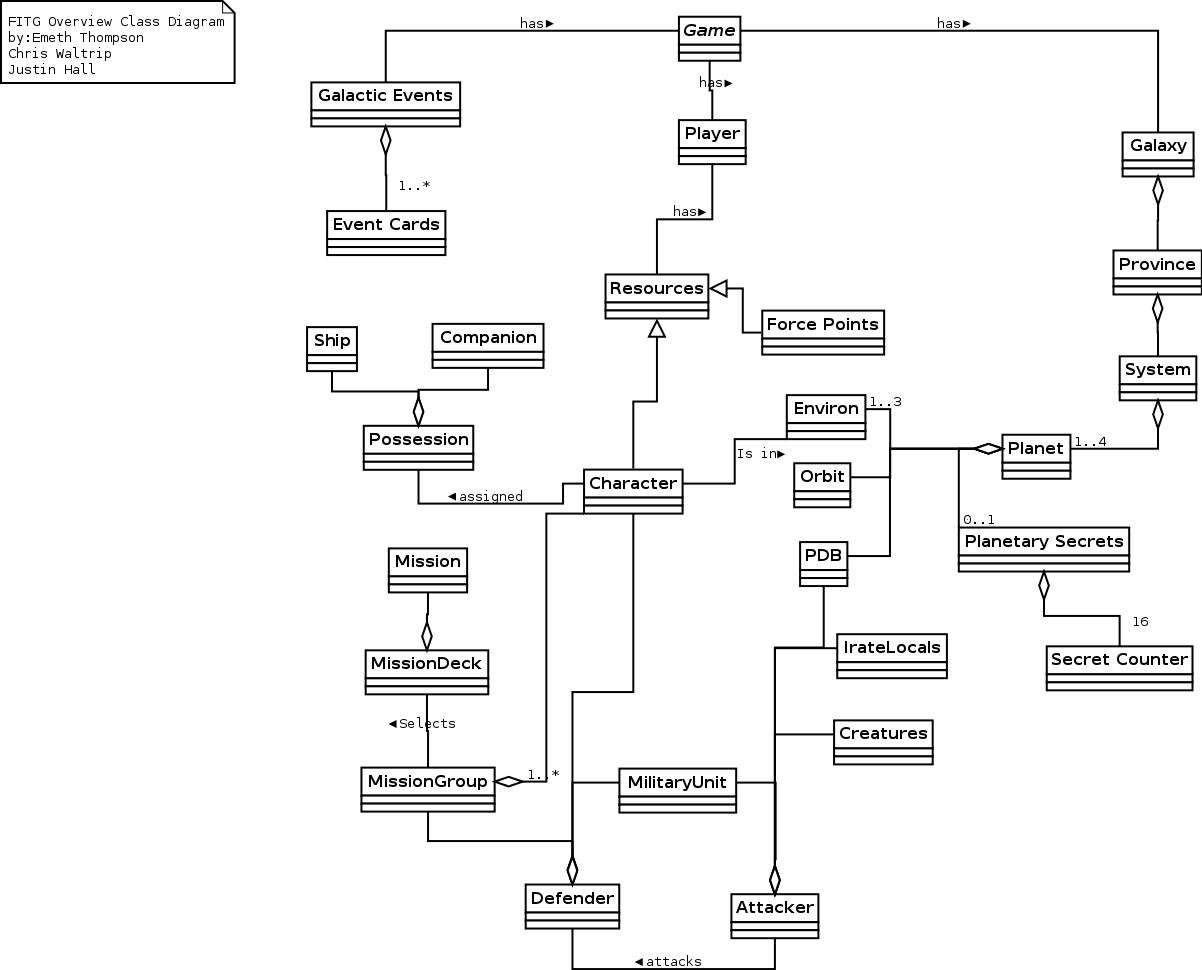
\includegraphics[width=\textwidth,height=\textheight,keepaspectratio]{./images/overview}
	\pagebreak
\pagebreak
\section{Class Diagrams}
	\subsection{Character Combat}
	\begin{tabularx}{\linewidth}{rcX}
				Written by & : & Ranger Adams, Sean Harris \\
				Reviewed by & : & Justin Hall, Emeth Thompson, Chris Waltrip  
	\end{tabularx}
		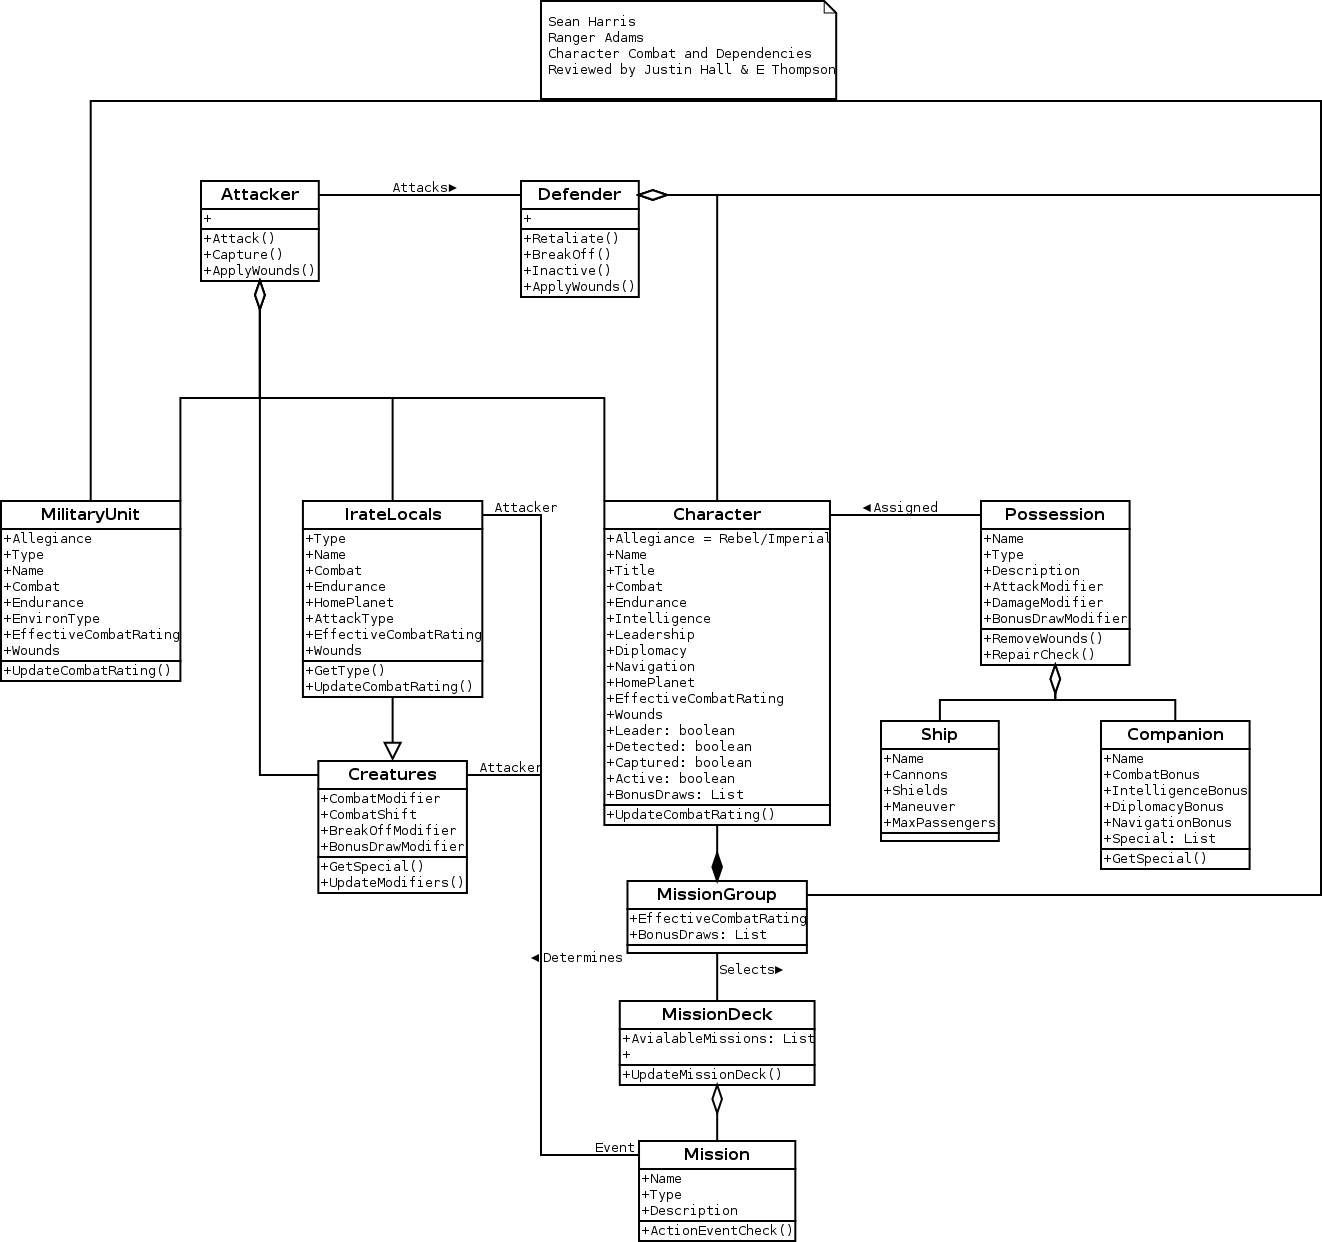
\includegraphics[width=\textwidth,height=\textheight,keepaspectratio]{./images/character_combat}
	\pagebreak
	\subsection{Galactic Events}
	\begin{tabularx}{\linewidth}{rcX}
				Written by & : & Paul Bailey, Joe Matranga \\
				Reviewed by & : & Justin Hall, Emeth Thompson, Chris Waltrip  
	\end{tabularx}
		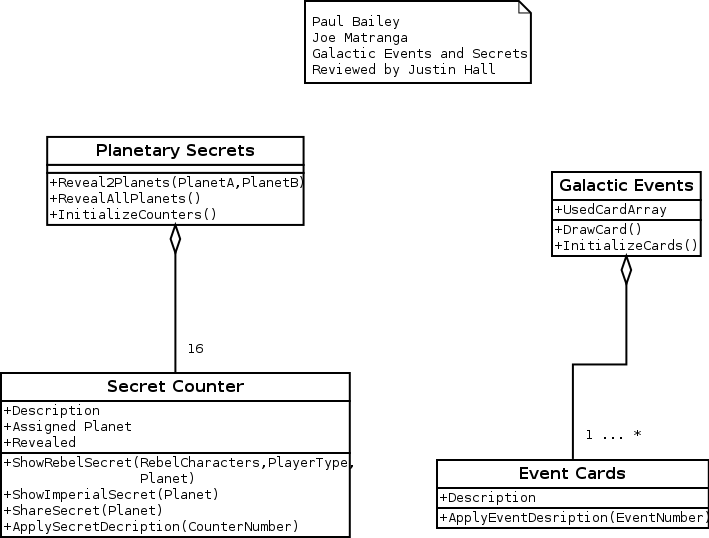
\includegraphics[width=\textwidth,height=\textheight,keepaspectratio]{./images/galactic_events}	
		\pagebreak
		
	\subsection{Galactic State}
	\begin{tabularx}{\linewidth}{rcX}
				Written by & : & Jeff Crocker, Ben Cumber \\
				Reviewed by & : & Justin Hall, Emeth Thompson, Chris Waltrip \\
				Reviewer notes & : & Gave feedback regarding some of the classes and how they were organized.  Everyone agreed on changes and they were made. 
	\end{tabularx}
		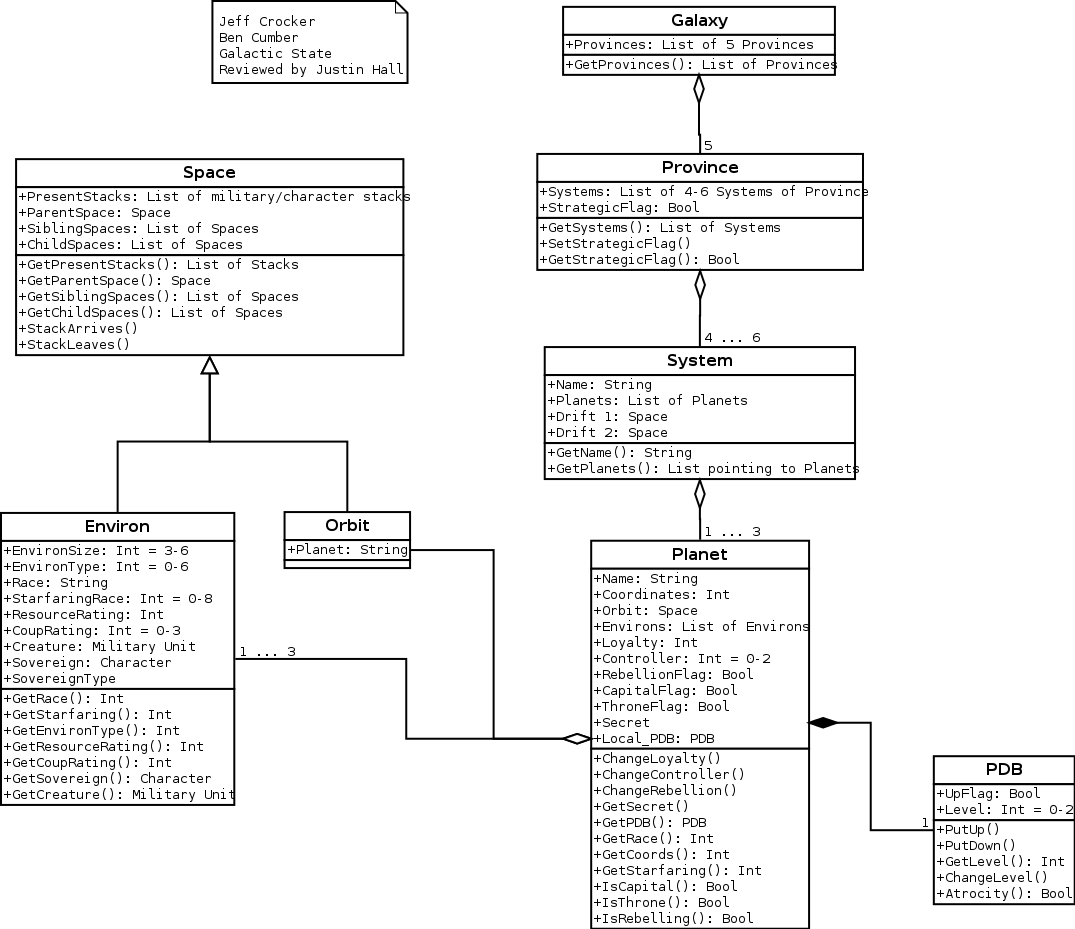
\includegraphics[width=\textwidth,height=\textheight,keepaspectratio]{./images/galactic_state}
		\pagebreak	
	\subsection{Military Combat and Military Units}
	\begin{tabularx}{\linewidth}{rcX}
				Written by & : & Sam Foster, Andy Schwartzmeyer \\
				Reviewed by & : & Justin Hall, Emeth Thompson, Chris Waltrip \\
				Reviewer notes & : & The reviewers felt that what was done was not a class diagram, but more of an object/flow/activity diagram.  This feedback was contested by one member and no changes have been made as of yet.
	\end{tabularx}
		\subsubsection{Military Units Class Diagram}
		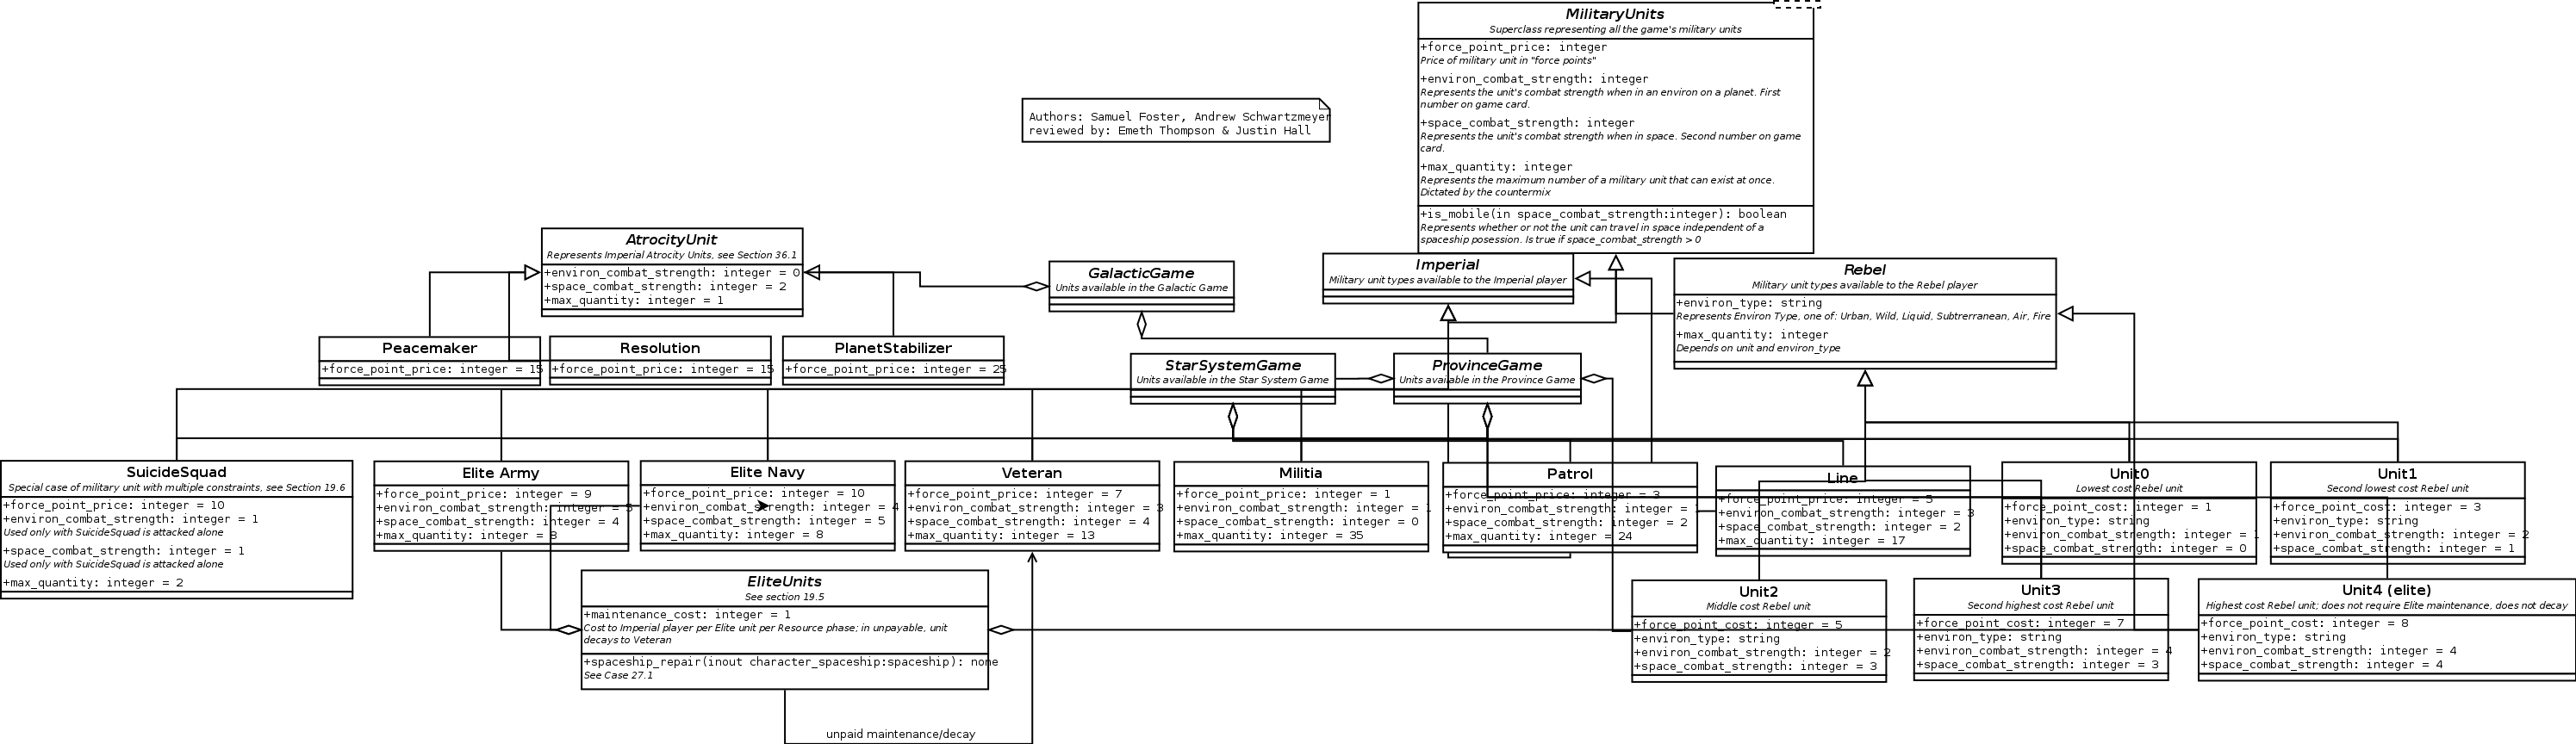
\includegraphics[width=\textwidth,height=\textheight,keepaspectratio]{./images/military_units}
		
		\pagebreak
		\subsubsection{Military Combat Class Diagram}
		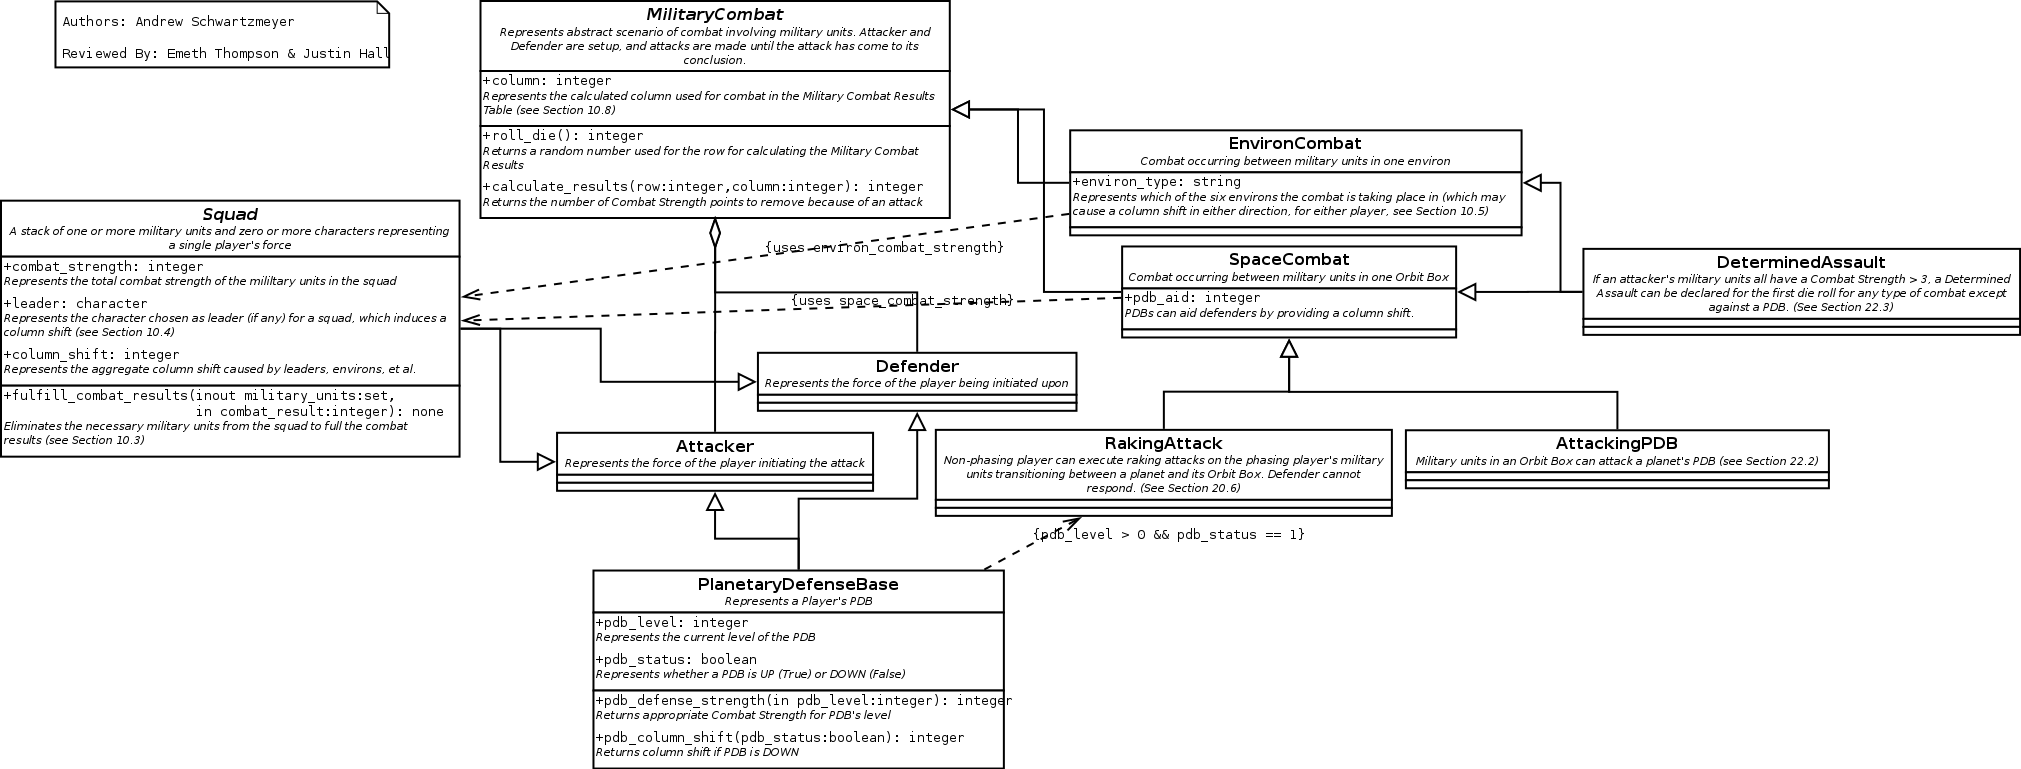
\includegraphics[width=\textwidth,height=\textheight,keepaspectratio]{./images/military_combat}
		
		\pagebreak
	\subsection{Missions}
	\begin{tabularx}{\linewidth}{rcX}
				Written by & : & Robert Meine, Greg Donaldson \\
				Reviewed by & : & Justin Hall, Emeth Thompson, Chris Waltrip \\
				Reviewer notes & : & The diagram initially didn't use the correct diagrams, but was fixed promptly. 
	\end{tabularx}
		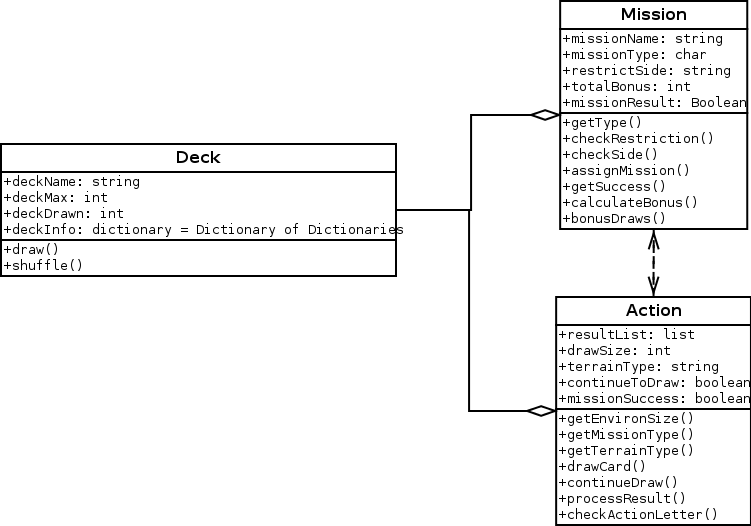
\includegraphics[width=\textwidth,height=\textheight,keepaspectratio]{./images/missions}
			\pagebreak
	\subsection{Resources and Taxation}
	\begin{tabularx}{\linewidth}{rcX}
				Written by & : & Jordan Leithart, Tao Zhan, Shaung Wang \\
				Reviewed by & : & Justin Hall, Emeth Thompson, Chris Waltrip \\
				Reviewer notes & : & Initially looked great, but a subsequent review found issues at the last minute that wouldn't have had time to have been changed yet.
	\end{tabularx}
		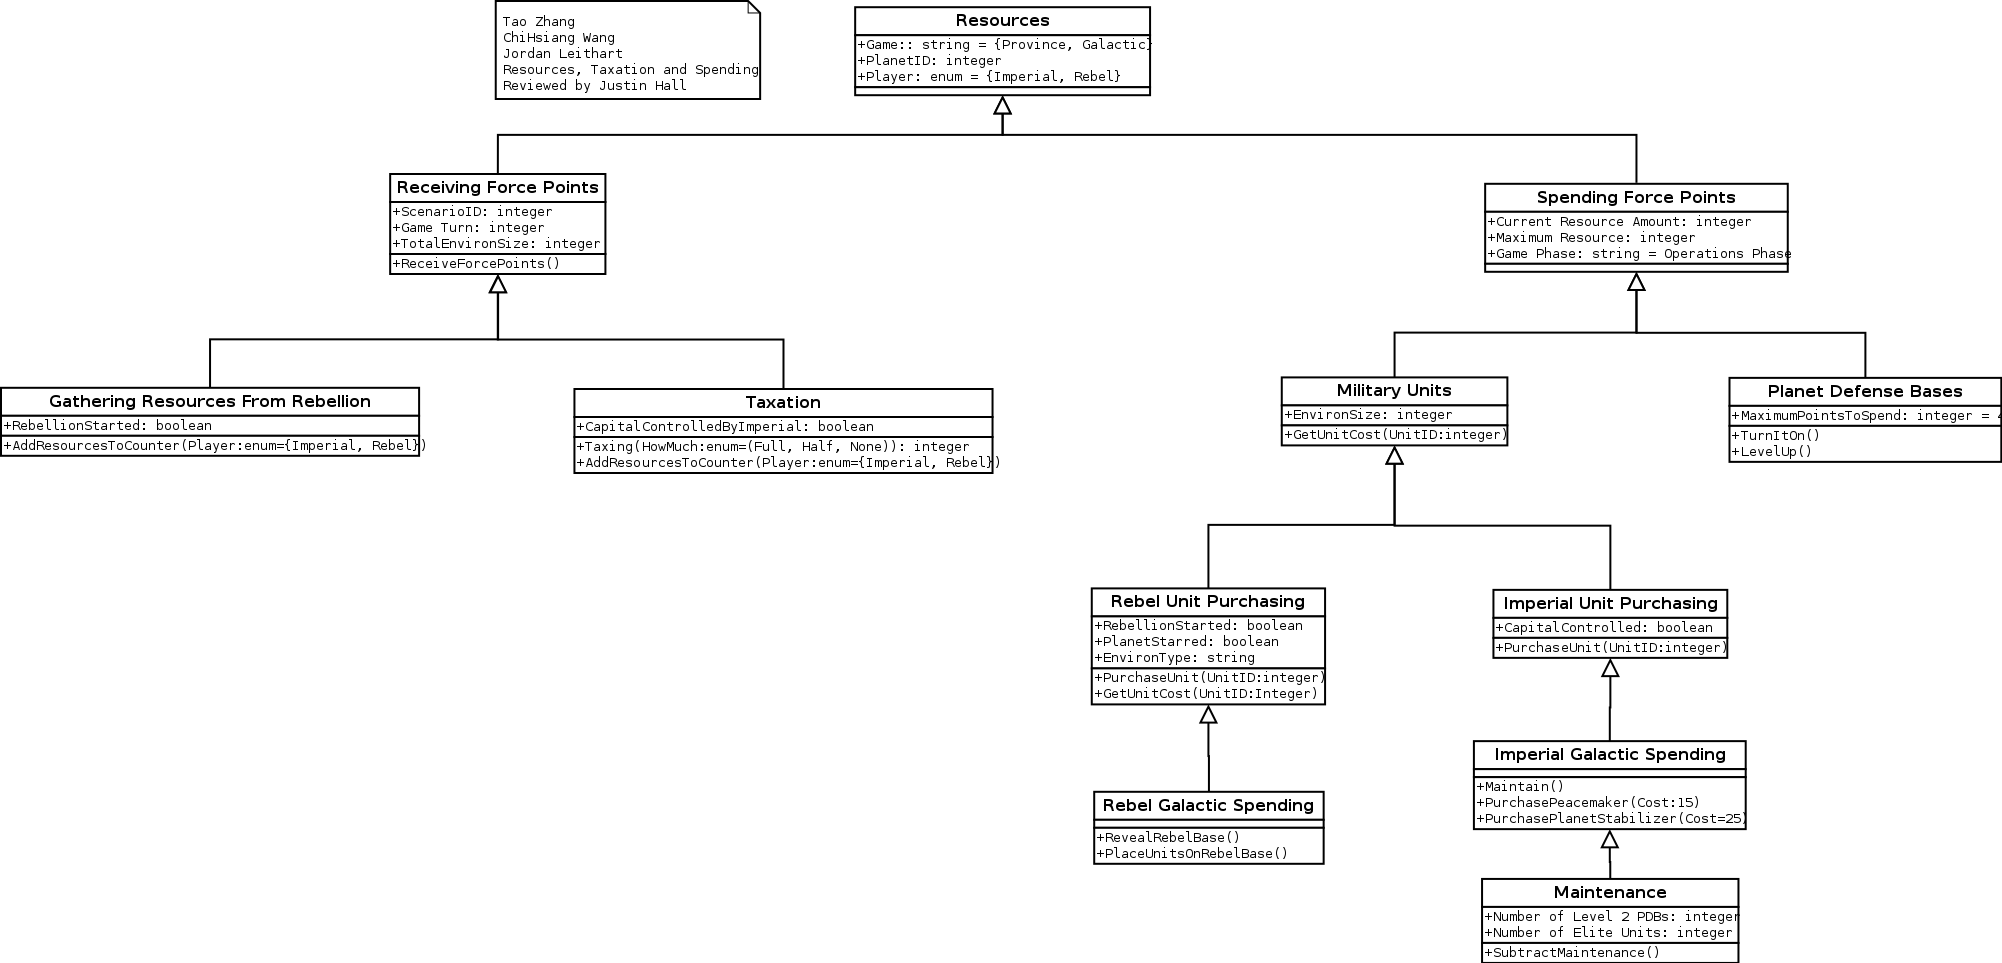
\includegraphics[width=\textwidth,height=\textheight,keepaspectratio]{./images/resources_taxation}



\end{document}